% !TEX program = xelatex
\documentclass[11pt, a4paper]{article}

\usepackage{fontspec}
\usepackage{xetexko}
\usepackage[margin=2cm, top=2.5cm, bottom=2.5cm]{geometry}
\usepackage{graphicx}
\usepackage{booktabs}
\usepackage{tabularx}
\usepackage{xcolor}
\usepackage{hyperref}
\usepackage{titlesec}
\usepackage{fancyhdr}
\usepackage{enumitem}
\usepackage{float}
\usepackage{caption}
\usepackage{array}
\usepackage{colortbl}
\usepackage{tikz}

\setmainfont{Apple SD Gothic Neo}
\setsansfont{Apple SD Gothic Neo}
\setmonofont{Menlo}

\definecolor{darkblue}{HTML}{1A5276}
\definecolor{medblue}{HTML}{2980B9}
\definecolor{lightblue}{HTML}{D4E6F1}
\definecolor{darkgray}{HTML}{2C3E50}
\definecolor{green}{HTML}{27AE60}
\definecolor{orange}{HTML}{E67E22}
\definecolor{red}{HTML}{E74C3C}

\hypersetup{colorlinks=true, linkcolor=darkblue, urlcolor=medblue}

\titleformat{\section}
  {\Large\bfseries\color{darkblue}}{\thesection.}{0.5em}{}
  [\vspace{-0.5em}\textcolor{medblue}{\rule{\textwidth}{0.5pt}}]
\titleformat{\subsection}
  {\large\bfseries\color{darkblue}}{\thesubsection}{0.5em}{}

\pagestyle{fancy}
\fancyhf{}
\fancyhead[L]{\small\color{darkgray}AI 기반 프랜차이즈 분석}
\fancyhead[R]{\small\color{darkgray}한양대 빅데이터마케팅 랩}
\fancyfoot[C]{\small\color{darkgray}\thepage}
\renewcommand{\headrulewidth}{0.4pt}

\newcolumntype{L}[1]{>{\raggedright\arraybackslash}p{#1}}
\newcolumntype{C}[1]{>{\centering\arraybackslash}p{#1}}

\setlength{\parskip}{4pt}

\begin{document}

% ── COVER ──
\thispagestyle{empty}
\begin{center}
\vspace*{2cm}

{\fontsize{28}{34}\selectfont\bfseries\color{darkblue}
배달은 리뷰가, 매장식사는 입지가\\[10pt]
매출을 결정합니다.}

\vspace{0.8cm}

{\Large\color{darkgray}
프랜차이즈 349개 매장 · 3년 데이터 · 채널별 매출 예측 \& 상권 분석}

\vspace{0.6cm}
\textcolor{medblue}{\rule{10cm}{0.8pt}}
\vspace{1.5cm}

\begin{tikzpicture}
\node[fill=lightblue, rounded corners=8pt, minimum width=15.5cm, minimum height=3.5cm] {
  \begin{minipage}{14.5cm}
  \centering
  \vspace{4pt}
  \begin{minipage}[t]{0.24\textwidth}\centering
    {\fontsize{26}{30}\selectfont\bfseries\color{darkblue}349개}\\[2pt]
    {\small\color{darkgray}매장 전수 분석}
  \end{minipage}\hfill
  \begin{minipage}[t]{0.24\textwidth}\centering
    {\fontsize{26}{30}\selectfont\bfseries\color{green}3년}\\[2pt]
    {\small\color{darkgray}주간 거래 데이터}
  \end{minipage}\hfill
  \begin{minipage}[t]{0.24\textwidth}\centering
    {\fontsize{26}{30}\selectfont\bfseries\color{darkblue}3채널}\\[2pt]
    {\small\color{darkgray}배달·매장·포장 분리}
  \end{minipage}\hfill
  \begin{minipage}[t]{0.24\textwidth}\centering
    {\fontsize{26}{30}\selectfont\bfseries\color{red}96\%}\\[2pt]
    {\small\color{darkgray}매장식사 예측 정확도}
  \end{minipage}
  \vspace{4pt}
  \end{minipage}
};
\end{tikzpicture}

\vspace{1cm}

\begin{minipage}{0.9\textwidth}
\colorbox{lightblue}{%
\begin{minipage}{\textwidth}\vspace{8pt}
\centering
\begin{minipage}{0.85\textwidth}
{\color{darkgray}
이 프로젝트에서는 프랜차이즈 349개 매장의 매출을 채널별(배달·매장식사·포장)로 분리하여 예측하고, \textbf{각 채널에서 매출을 결정하는 요인이 완전히 다르다}는 것을 밝혔습니다. 배달은 리뷰와 1인 가구에, 매장식사는 입지와 경쟁에 좌우됩니다.}
\end{minipage}
\vspace{8pt}
\end{minipage}%
}
\end{minipage}

\vspace{2cm}

{\large\color{darkgray}
한양대학교 경영대학 · 빅데이터마케팅 랩 · 임보람 교수\\[4pt]
brlim@hanyang.ac.kr · bigdatamarketinglab.com}
\end{center}

\newpage

% ═══════════════════════════════════════════════════════
\section{프랜차이즈 본사가 데이터로 답할 수 있는 질문}

\begin{table}[H]
\centering
\renewcommand{\arraystretch}{1.5}
\begin{tabularx}{\textwidth}{C{0.8cm} L{5cm} X}
\toprule
\rowcolor{lightblue} & \textbf{질문} & \textbf{AI가 답하는 방식} \\
\midrule
\textbf{1} & \textbf{이 매장의 다음 달 매출은?} & 채널별(배달/매장식사/포장) 각각의 매출을 예측합니다. 매장식사 96\%, 배달 78\%의 정확도. \\[4pt]
\textbf{2} & \textbf{어디에 매장을 내야 하나?} & 후보지의 인구 구성, 경쟁사, 자사 매장 거리를 분석하여 채널별 예상 매출을 산출합니다. \\[4pt]
\textbf{3} & \textbf{배달에 집중할까, 매장식사에 집중할까?} & 해당 지역의 1인 가구 비율이 높으면 배달, 고령 인구가 많으면 매장식사 — 데이터로 판단합니다. \\[4pt]
\textbf{4} & \textbf{우리 매장끼리 매출을 나눠먹고 있진 않나?} & 자기잠식(cannibalization) 분석. 100m 이내 같은 브랜드 매장이 가장 큰 매출 감소를 유발합니다. \\[4pt]
\textbf{5} & \textbf{리뷰 관리를 어떻게 해야 하나?} & 별점이 아니라 ``음식이 맛있다''는 \textbf{구체적 언급}이 배달 매출과 직결됩니다. \\[4pt]
\textbf{6} & \textbf{이 매장, 위험하지 않나?} & 매출 하락 추세를 사전에 탐지. 특정 채널의 매출이 먼저 떨어지는 패턴을 감지합니다. \\
\bottomrule
\end{tabularx}
\end{table}

\newpage

% ═══════════════════════════════════════════════════════
\section{핵심 발견: 배달과 매장식사는 완전히 다른 게임이다}

같은 브랜드, 같은 매장인데, 채널에 따라 매출을 결정하는 요인이 \textbf{정반대}입니다. 349개 매장의 3년 데이터를 분석한 결과입니다.

\begin{figure}[H]
\centering
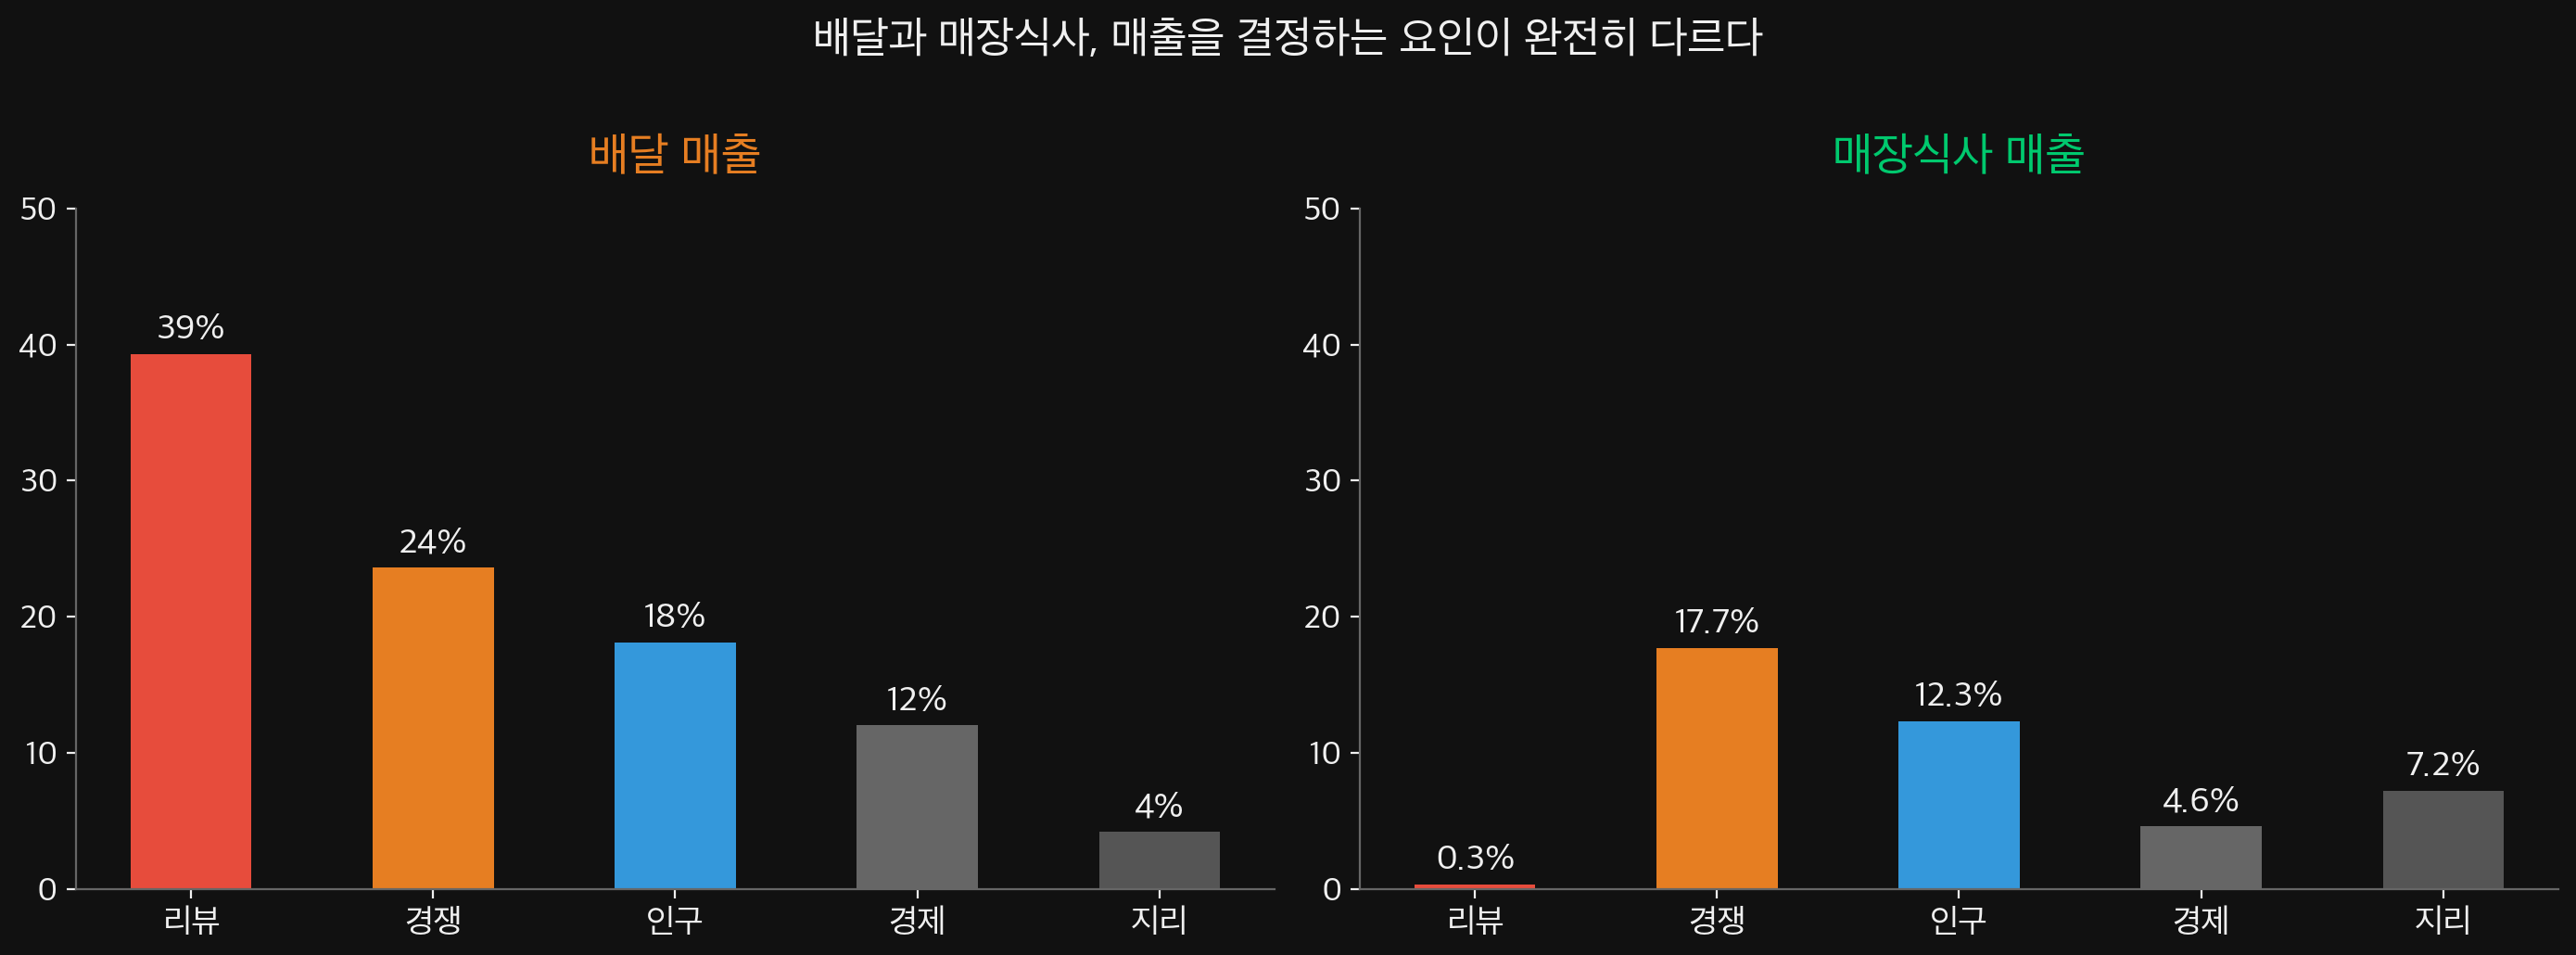
\includegraphics[width=0.9\textwidth]{bbq_channel_comparison.png}
\caption{배달 매출과 매장식사 매출, 결정 요인이 완전히 다르다}
\end{figure}

\begin{table}[H]
\centering
\renewcommand{\arraystretch}{1.4}
\large
\begin{tabular}{L{4cm} C{5cm} C{5cm}}
\toprule
\rowcolor{lightblue} & \textbf{배달} & \textbf{매장식사} \\
\midrule
\textbf{1위 요인} & \textcolor{red}{\textbf{리뷰 (39.3\%)}} & \textcolor{orange}{\textbf{경쟁 환경 (17.7\%)}} \\[4pt]
\textbf{2위 요인} & 경쟁 (23.6\%) & 인구·상권 (12.3\%) \\[4pt]
\textbf{리뷰 영향} & \textcolor{red}{\textbf{압도적}} & 거의 없음 (0.3\%) \\[4pt]
\textbf{핵심 인구 변수} & 1인 가구 비율 & 고령화 지수 \\[4pt]
\textbf{의미} & 리뷰 관리 + 1인 가구 타겟 & 입지 선정이 전부 \\
\bottomrule
\end{tabular}
\caption{채널별 매출 결정 요인 비교 (XGBoost + SHAP 기반 분석)}
\end{table}

\colorbox{lightblue}{%
\begin{minipage}{0.95\textwidth}\vspace{8pt}
\textbf{시사점:} 배달 중심 매장과 매장식사 중심 매장의 운영 전략이 달라야 합니다. 같은 브랜드라도 지역 특성에 따라 채널 비중이 다르고, 매출을 올리는 방법도 다릅니다. 이것을 하나의 전략으로 관리하면 기회를 놓칩니다.
\vspace{8pt}
\end{minipage}%
}

\newpage

% ═══════════════════════════════════════════════════════
\section{출점 전략: 1인 가구 밀도가 배달 매출을 결정한다}

``유동인구가 많은 곳에 매장을 내라'' — 배달 시대에 이 공식은 더 이상 작동하지 않습니다.

349개 매장 분석 결과, 배달 매출을 가장 강력하게 예측하는 인구 변수는 \textbf{1인 가구 비율}이었습니다. 유동인구는 배달 매출과 거의 관련이 없었습니다.

\begin{table}[H]
\centering
\renewcommand{\arraystretch}{1.3}
\begin{tabularx}{\textwidth}{L{5cm} C{3cm} X}
\toprule
\rowcolor{lightblue} \textbf{변수} & \textbf{기여도} & \textbf{해석} \\
\midrule
\textbf{1인 가구 비율} & \textcolor{red}{\textbf{5.2\%}} & 혼자 사는 사람은 배달에 의존. 구조적 수요. \\[4pt]
\textbf{반경 1km 인구} & 3.1\% & 많으면 좋지만, 1인 가구 비율보다 중요도 낮음 \\[4pt]
\textbf{고령화 지수} & 3.0\% & 고령 인구 ↑ → 매장식사 ↑, 배달 ↓ \\[4pt]
\textbf{유동인구} & 낮음 & 배달은 집에서 시킴. 거리의 사람 수와 무관 \\
\bottomrule
\end{tabularx}
\caption{배달 매출 예측에서 인구 변수의 중요도 (SHAP 기반)}
\end{table}

\textbf{실무 원칙:}
\begin{itemize}[itemsep=4pt, leftmargin=2em]
  \item 배달 중심 출점: 1인 가구 밀집 지역 (대학가, 원룸 밀집 지역) 우선
  \item 매장식사 중심 출점: 고령 인구 비율이 높은 전통 상권
  \item 같은 도시 안에서도 구/동에 따라 최적 전략이 다름
\end{itemize}

\newpage

% ═══════════════════════════════════════════════════════
\section{자기잠식: 가장 위험한 경쟁자는 우리 브랜드다}

프랜차이즈 본사가 출점 시 가장 먼저 확인하는 것은 ``경쟁 브랜드 수''입니다. 하지만 데이터는 다른 이야기를 합니다.

\textbf{배달 매출에서, 타 브랜드보다 같은 브랜드의 다른 매장이 더 큰 매출 감소를 유발했습니다.}

\begin{figure}[H]
\centering
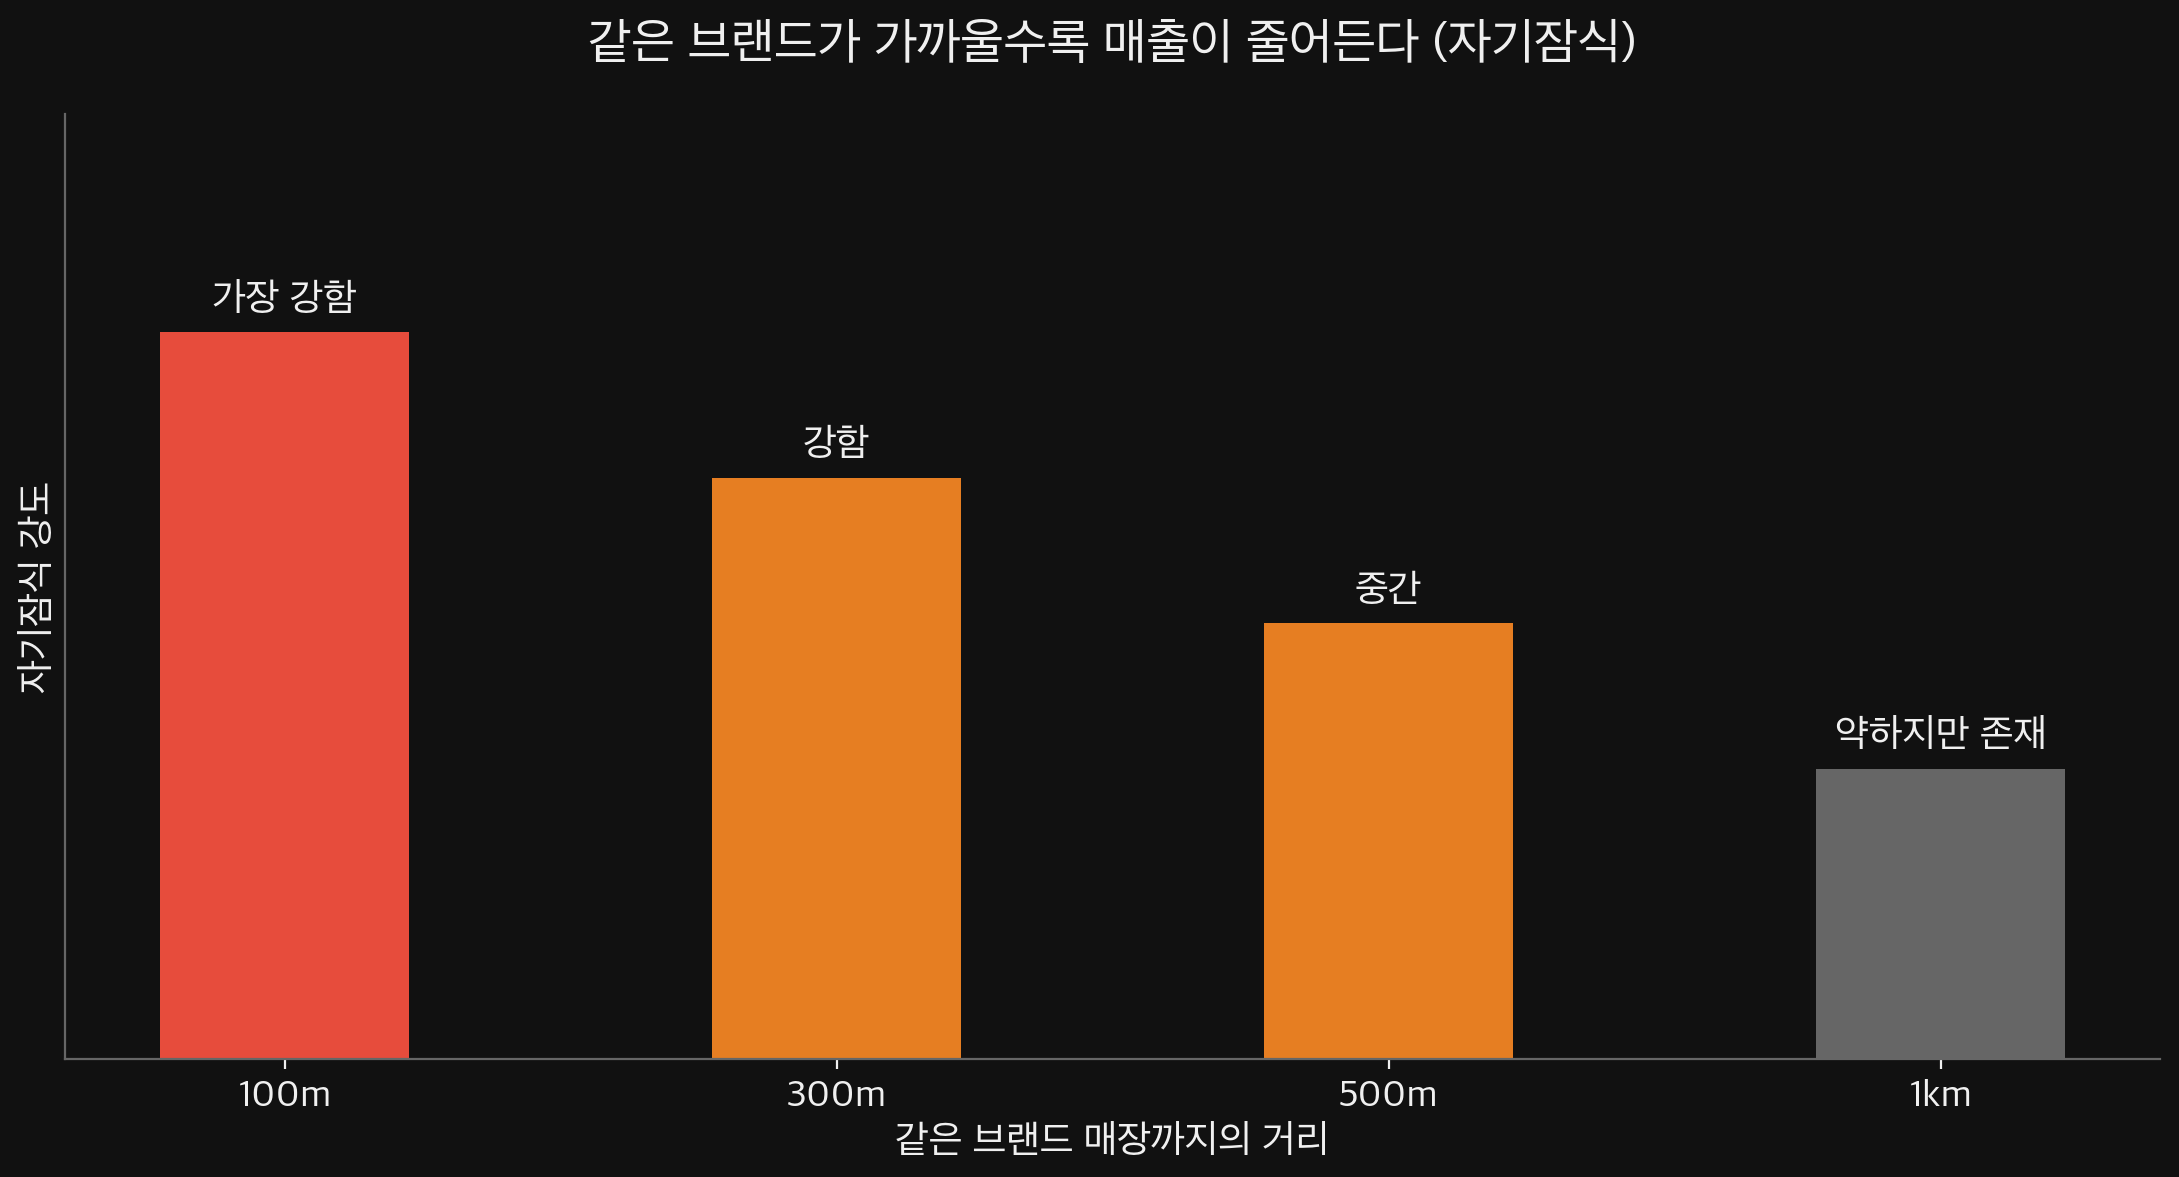
\includegraphics[width=0.8\textwidth]{bbq_cannibalization.png}
\caption{같은 브랜드 매장이 가까울수록 배달 매출이 줄어든다}
\end{figure}

\subsection{왜 자기잠식이 발생하는가}

배달앱을 열면, 반경 내 모든 매장이 한 화면에 동시에 뜹니다. 같은 브랜드의 A지점과 B지점은 메뉴가 같고, 가격이 같고, 프로모션도 같습니다. 소비자 입장에서 \textbf{완벽한 대체재}입니다.

타 브랜드(교촌 vs BBQ)는 최소한 메뉴와 맛이 다릅니다. 하지만 같은 브랜드끼리는 차별점이 없어서, 배달 시간이 5분 빠른 쪽, 쿠폰이 있는 쪽을 누릅니다.

\textbf{매장식사에서는 이 자기잠식이 거의 나타나지 않았습니다.} 직접 방문하는 고객은 물리적으로 가까운 한 곳만 가기 때문입니다.

\colorbox{lightblue}{%
\begin{minipage}{0.95\textwidth}\vspace{8pt}
\textbf{실무 시사점:}
\begin{itemize}[itemsep=3pt, leftmargin=1.5em]
  \item ``경쟁 브랜드가 몇 개인가''보다 ``우리 매장이 이미 있는가''를 먼저 확인
  \item 배달 중심 매장은 자사 매장 간 배달 반경 중복을 본사 차원에서 관리해야 함
  \item 본사의 가맹점 확대 전략과 개별 가맹점 수익성이 충돌할 수 있는 구조적 이슈
\end{itemize}
\vspace{4pt}
\end{minipage}%
}

\newpage

% ═══════════════════════════════════════════════════════
\section{리뷰 관리: ``맛있다''가 매출과 직결된다}

``리뷰가 매출에 영향을 미친다''는 건 상식처럼 들립니다. 하지만 데이터는 더 정밀한 이야기를 합니다.

GPT-4 기반 자연어 분석으로 리뷰를 4가지 주제(음식 품질, 서비스, 가격, 재구매 의향)로 분류하고, 각 주제가 매출에 미치는 영향을 측정했습니다.

\begin{figure}[H]
\centering
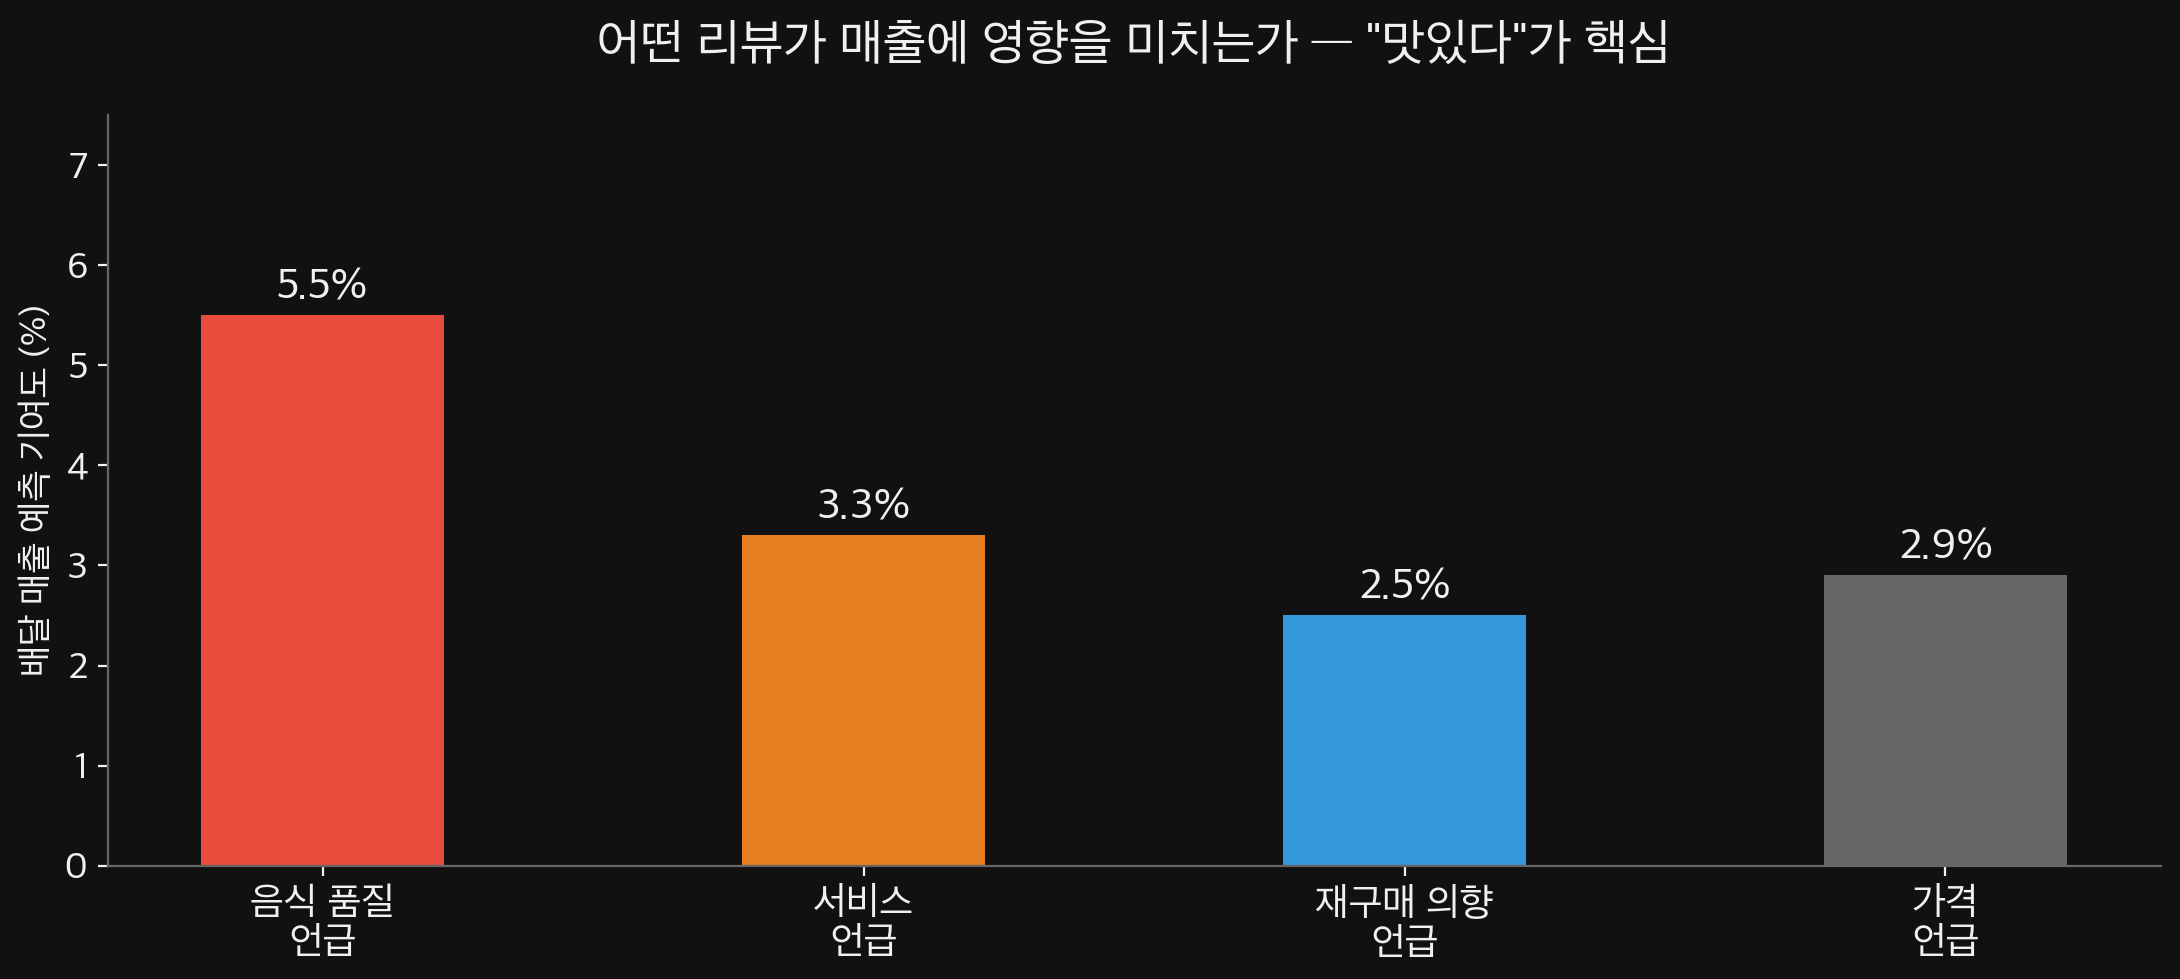
\includegraphics[width=0.8\textwidth]{bbq_review_impact.png}
\caption{리뷰 주제별 배달 매출 예측 기여도 — 음식 품질이 압도적}
\end{figure}

\begin{table}[H]
\centering
\renewcommand{\arraystretch}{1.3}
\begin{tabularx}{\textwidth}{L{4cm} C{3cm} X}
\toprule
\rowcolor{lightblue} \textbf{리뷰 주제} & \textbf{기여도} & \textbf{해석} \\
\midrule
\textbf{음식 품질 언급} & \textcolor{red}{\textbf{5.5\%}} & ``치킨이 바삭하다'' — 가장 강력 \\[4pt]
서비스 언급 & 3.3\% & ``배달이 빠르다'' — 보조적 \\[4pt]
가격 언급 & 2.9\% & ``가성비 좋다'' — 중간 \\[4pt]
재구매 의향 & 2.5\% & ``또 시킬게요'' — 약함 \\
\bottomrule
\end{tabularx}
\end{table}

\textbf{중요:} 매장식사 매출에서 리뷰의 영향은 \textbf{거의 0}이었습니다 (기여도 0.3\%). 직접 방문하는 고객은 리뷰 대신 자기 경험을 기준으로 판단하기 때문입니다.

\colorbox{lightblue}{%
\begin{minipage}{0.95\textwidth}\vspace{8pt}
\textbf{실무 시사점:}
\begin{itemize}[itemsep=3pt, leftmargin=1.5em]
  \item 배달 매출을 올리려면 ``별점 4.5 이상 유지''가 아니라, \textbf{``맛있다''는 구체적 언급을 늘리는 것}이 핵심
  \item 리뷰 이벤트보다 ``치킨의 바삭함은 어떠셨나요?'' 같은 \textbf{유도 질문}이 효과적
  \item 매장식사 중심 매장은 리뷰 관리에 과투자하지 말 것 — 입지가 더 중요
\end{itemize}
\vspace{4pt}
\end{minipage}%
}

\newpage

% ═══════════════════════════════════════════════════════
\section{채널별 매출 예측 정확도}

349개 매장의 3년 주간 거래 데이터를 학습하고, \textbf{학습에 쓰지 않은 미래 기간}으로만 검증한 결과입니다.

\begin{figure}[H]
\centering
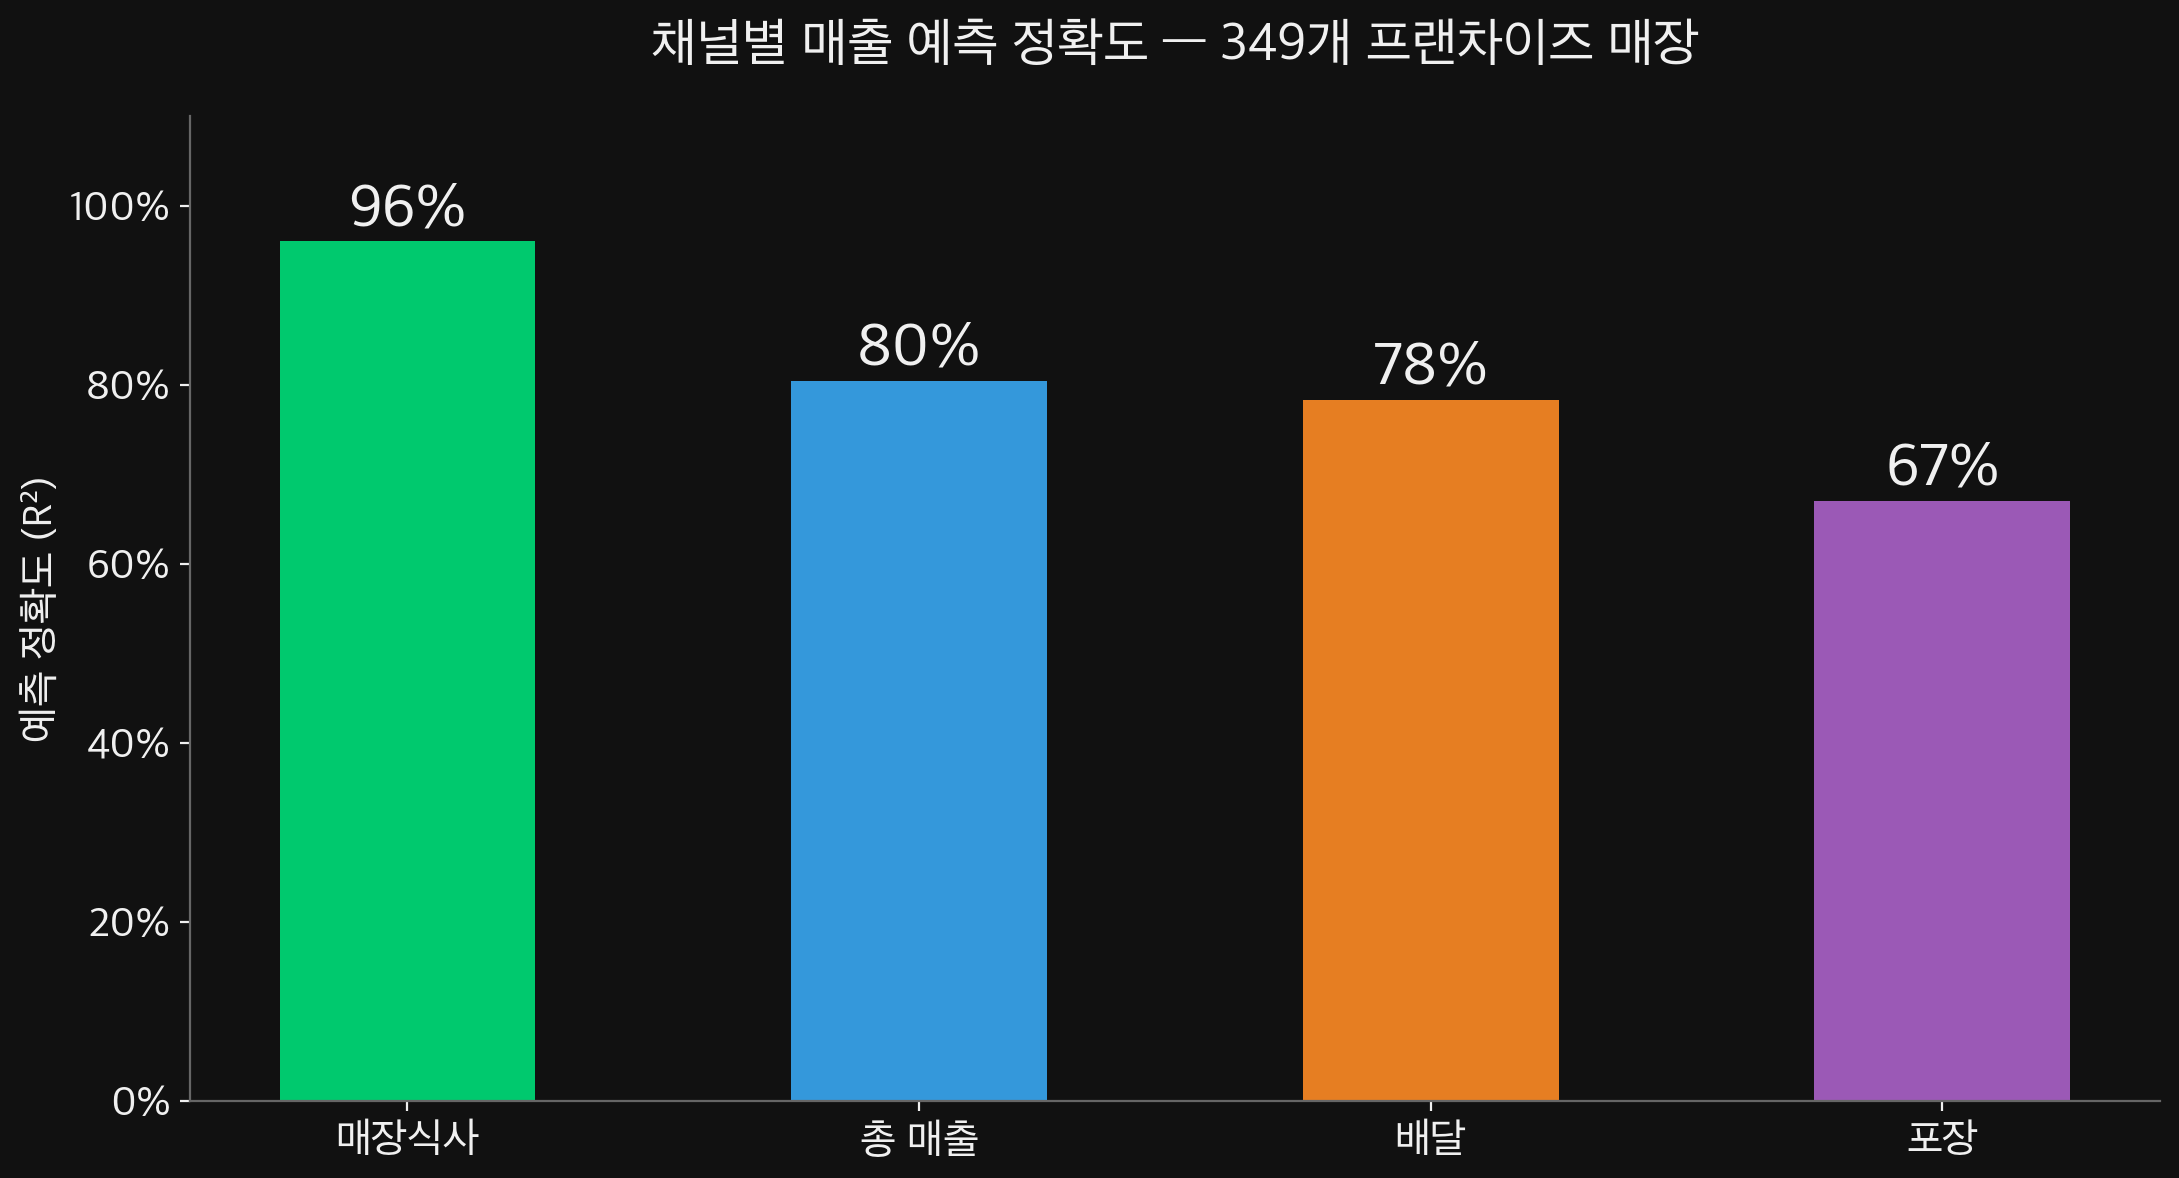
\includegraphics[width=0.8\textwidth]{bbq_channel_accuracy.png}
\caption{채널별 매출 예측 정확도 (Out-of-sample, R²)}
\end{figure}

\begin{table}[H]
\centering
\renewcommand{\arraystretch}{1.3}
\large
\begin{tabular}{L{4cm} C{3cm} L{7cm}}
\toprule
\rowcolor{lightblue} \textbf{채널} & \textbf{정확도 (R²)} & \textbf{활용} \\
\midrule
\textbf{매장식사} & \textcolor{green}{\textbf{96\%}} & 매장별 인력 배치, 좌석 운영 최적화 \\[4pt]
\textbf{총 매출} & \textcolor{darkblue}{\textbf{80\%}} & 전체 매장 손익 관리, 임대료 협상 근거 \\[4pt]
\textbf{배달} & \textbf{78\%} & 배달 물량 예측, 포장재·식자재 발주 \\[4pt]
\textbf{포장} & 67\% & 포장 수요 대비 인력 배치 \\
\bottomrule
\end{tabular}
\end{table}

\textbf{예측에 사용한 데이터:}
\begin{itemize}[itemsep=3pt, leftmargin=2em]
  \item 상권 인구 특성 (1인 가구 비율, 인구 밀도, 고령화 지수)
  \item 경쟁 환경 (반경 100m$\sim$1km 타 브랜드 및 자사 매장 수)
  \item 온라인 리뷰 (GPT-4 기반 주제 분류 + 감성 분석)
  \item 거시 경제 (소비자물가, 가계소득, 실업률)
  \item 날씨 (기온, 강수량, 습도)
\end{itemize}

외부 데이터 구매 없이, \textbf{POS 데이터 + 공개 데이터}만으로 구축합니다.

\newpage

% ═══════════════════════════════════════════════════════
\section{종합: 프랜차이즈 본사를 위한 데이터 기반 의사결정}

\begin{table}[H]
\centering
\renewcommand{\arraystretch}{1.5}
\begin{tabularx}{\textwidth}{C{0.8cm} L{4cm} X L{3.5cm}}
\toprule
\rowcolor{lightblue} & \textbf{의사결정} & \textbf{지금} & \textbf{데이터 기반} \\
\midrule
\textbf{1} & 출점 위치 선정 & 부동산 중개인 + 감 & 인구 구성 분석 + 채널별 예상 매출 산출 \\[4pt]
\textbf{2} & 매장 채널 전략 & 전 매장 동일 전략 & 지역 특성에 따라 배달/매장식사 비중 최적화 \\[4pt]
\textbf{3} & 가맹점 추가 출점 & ``지역에 아직 여유 있다'' & 자기잠식 시뮬레이션 후 결정 \\[4pt]
\textbf{4} & 리뷰 관리 & 별점 올리기 & 음식 품질 구체적 언급 유도 \\[4pt]
\textbf{5} & 위험 매장 관리 & 매출 떨어진 후 대응 & 하락 추세 사전 탐지 + 원인 분석 \\[4pt]
\textbf{6} & 매장별 매출 예측 & 작년 동기 참고 & AI가 채널별로 각각 예측 \\
\bottomrule
\end{tabularx}
\end{table}

\vspace{0.5cm}

\colorbox{lightblue}{%
\begin{minipage}{0.95\textwidth}\vspace{8pt}
\centering
{\large\bfseries\color{darkblue} 데이터만 있으면 됩니다}\\[8pt]
\begin{minipage}{0.85\textwidth}
매장별 일간 또는 주간 POS 데이터(최소 1년). 배달/매장식사/포장 채널이 구분되면 채널별 분석 가능. 리뷰 데이터가 있으면 리뷰 영향 분석까지. 외부 데이터 구매 불필요 — 공개 데이터로 상권·인구·경쟁 변수를 구축합니다.
\end{minipage}
\vspace{8pt}
\end{minipage}%
}

\vspace{1.5cm}

\begin{center}
\textcolor{medblue}{\rule{8cm}{0.8pt}}

\vspace{0.8cm}

{\Large\bfseries\color{darkblue} 문의}

\vspace{0.4cm}

{\large\color{darkgray}
임보람 교수\\[3pt]
한양대학교 경영대학 · 빅데이터마케팅 랩\\[6pt]
brlim@hanyang.ac.kr\\[3pt]
bigdatamarketinglab.com}
\end{center}

\end{document}
